% !TEX TS-program = pdflatex
% !TEX encoding = UTF-8 Unicode


\documentclass[11pt]{article} % use larger type; default would be 10pt
\usepackage[utf8]{inputenc} % set input encoding (not needed with XeLaTeX)

%%%  defien variables and commands to use throughout the document
	\newcommand{\InsertTitle}{This is a Dummy Title of Great Importance}	
	\def\changemargin#1#2{\list{}{\rightmargin#2\leftmargin#1}\item[]} %Énable Margin Hacking where necessary	
	\let\endchangemargin=\endlist 
	\newcommand{\spacing}{\vspace{0.4cm}}
	

%%% PAGE DIMENSIONS
	\usepackage{geometry} % to change the page dimensions
	\geometry{a4paper} % or letterpaper (US) or a5paper or....
	% \geometry{margin=2in} % for example, change the margins to 2 inches all round

%%% PACKAGES
	\usepackage{graphicx} % support the \includegraphics command and options
	\usepackage{booktabs} % for much better looking tables
	\usepackage{array} % for better arrays (eg matrices) in maths
	\usepackage{paralist} % very flexible & customisable lists (eg. enumerate/itemize, etc.)
	\usepackage{verbatim} % adds environment for commenting out blocks of text & for better verbatim
	\usepackage{subfig} % make it possible to include more than one captioned figure/table in a single float
	\usepackage[english, german]{babel} %german support
	\usepackage[T1]{fontenc}
	\usepackage{blindtext}	%insert blind texts
	\usepackage{helvet}	%use helvetica, arial no available
	\usepackage{float} % for prettier float
	\usepackage[table,xcdraw]{xcolor}  % for colorful tables
	\usepackage[titletoc,toc,title,page]{appendix} % Anhang 
	\usepackage{chngcntr} % to change to eper chapter counter
	\usepackage{cite}	%cite from bibtex
	\usepackage{url}	%use urls in citing
	\usepackage[parfill]{parskip} %insert blank line, no indent on paragraphs
	\usepackage{multirow} %use multiple rows
	\usepackage{multicol}
	\usepackage{wrapfig} %to wrap figures
%	\usepackage{tocloft}
%\renewcommand{\appendixpagename}{\appendixname} %
%\renewcommand{\appendixtocname}{\appendixname} 
	


%%% HEADERS & FOOTERS
	\usepackage{fancyhdr} % This should be set AFTER setting up the page geometry

	\fancyhf{}
	\lhead{\leftmark}
	\chead{}
	\rhead{
\includegraphics[width=1cm]{icon.png}}

	\lfoot{\InsertTitle}
	\cfoot{}
	\rfoot{\thepage}

	\renewcommand{\headrulewidth}{1pt}
	\renewcommand{\footrulewidth}{1pt}

	\fancypagestyle{noheader}{
 		 \fancyhf{}% Clear header/footer
		\setlength{\headsep}{1.5cm}
		\lhead{\leftmark}
 		 \chead{}
		\rhead{
\includegraphics[width=1cm]{icon.png}}
	
		\lfoot{\InsertTitle}
		\cfoot{}
		\rfoot{\thepage}

		\renewcommand{\headrulewidth}{1pt}
		\renewcommand{\footrulewidth}{1pt}
	}

%%% Floatstyle
	\floatstyle{boxed}   %box around figure
	\restylefloat{figure}

	\floatstyle{plaintop} 
	\restylefloat{table}

	\counterwithin{figure}{section}
	\counterwithin{table}{section}

	\captionsetup{justification=raggedright,singlelinecheck=false}


%%% SECTION TITLE APPEARANCE
	\usepackage{sectsty}
	\allsectionsfont{\sffamily\mdseries\upshape} % (See the fntguide.pdf for font help)


%%% ToC (table of contents) APPEARANCE
	\usepackage[nottoc,notlof,notlot]{tocbibind} % Put the bibliography in the ToC
	\usepackage[titles,subfigure]{tocloft} % Alter the style of the Table of Contents
	%\renewcommand{\cftsecfont}{\rmfamily\mdseries\upshape}
	%\renewcommand{\cftsecpagefont}{\rmfamily\mdseries\upshape} % No bold!

%%% Set font to the font installed in usepackage
	\renewcommand{\familydefault}{\sfdefault}	

%%% Set page style
	\pagestyle{fancy} % options: empty , plain , fancy


%%% END Article customizations

%%% Begin Document


\begin{document}

%% Titelblatt
\begin{titlepage}
	\thispagestyle{empty}
	\centering
	% Title Graphic
	
\includegraphics[width=0.4\textwidth]{title.png}\par\vspace{1cm}
	% Title Header
	{\scshape Betriebliche Projektarbeit  \\}
	{\scshape Projektdokumentation  \par}
	%\vspace{0.5cm}
	 % Title
	\begin{changemargin}{0cm}{0cm}
	\centering
	{\huge\bfseries \InsertTitle \par}
	\end{changemargin} 
	%\vspace{0.1cm}
	% Icon
	
\includegraphics[width=0.1\textwidth]{icon.png}
	%\vfill
	\vspace{0.5cm}
	 % Info Block
	 \vfill
%\begin{multicols}{2}
%\setlength{\columnsep}{0cm}
	\begin{changemargin}{0cm}{0cm}
	\raggedright
	{\bfseries Vorgelegt von:\\}
	Peter Jan Eggert Gumrich\\
	Fast Lane GmbH \\
	Gasstr 4a \\
	22761 Hamburg \\ 
	\spacing
	{\bfseries Prüflingsnummer:\\}
	23423423423432r\\	
	\spacing	
	{\bfseries Ausbildungsberuf:\\}
	Fachinformatiker - Systemintegration\\
%	\columnbreak
	\spacing
	{\bfseries Ausbilder:\\}
	Boris Böttcher\\
	Fast Lane  GmbH \\
	Gasstr 4a\\
	\spacing
	{\bfseries Abgabedatum:\\}
	23.04.2019\\
	\end{changemargin} 
%\end{multicols}
	\vfill
	% Bottom of the page	
\end{titlepage}


%% TOC
\newpage
\pagenumbering{roman}
%\thispagestyle{fancy}
\thispagestyle{noheader}
\tableofcontents 
\newpage

%% Einleitung
\pagenumbering{arabic}
\section*{Einleitung}
	\addcontentsline{toc}{section}{Einleitung}
	\markboth{EINLEITUNG}{}
	\blindtext
		\par
	\blindtext
	\par
	Ich zitiere \cite{SomeWebsite}

%% Erster Abschnitt
\section{First section}
	\blindtext
	\blindlist{enumerate}[5]
	\subsection{First subsection}
		\blindtext
		\begin{table}[]
		
		\begin{tabular}{|l|l|l|l|l}
		\cline{1-4}
		sd  & sds  & sd   & sd   &  \\ \cline{1-4}
		sad & sda  & sad  & aS   &  \\ \cline{1-4}
		asa & aS   & As   & as   &  \\ \cline{1-4}
		aSA & Asas & aSAS & ASAs &  \\ \cline{1-4}
		\end{tabular}
		\caption{This table shows some data}
	  	\label{tab:myfirsttable}
		\end{table}
	
	\subsection{Second subsection}
		\blindtext
		\begin{figure}[h]
		\centering
		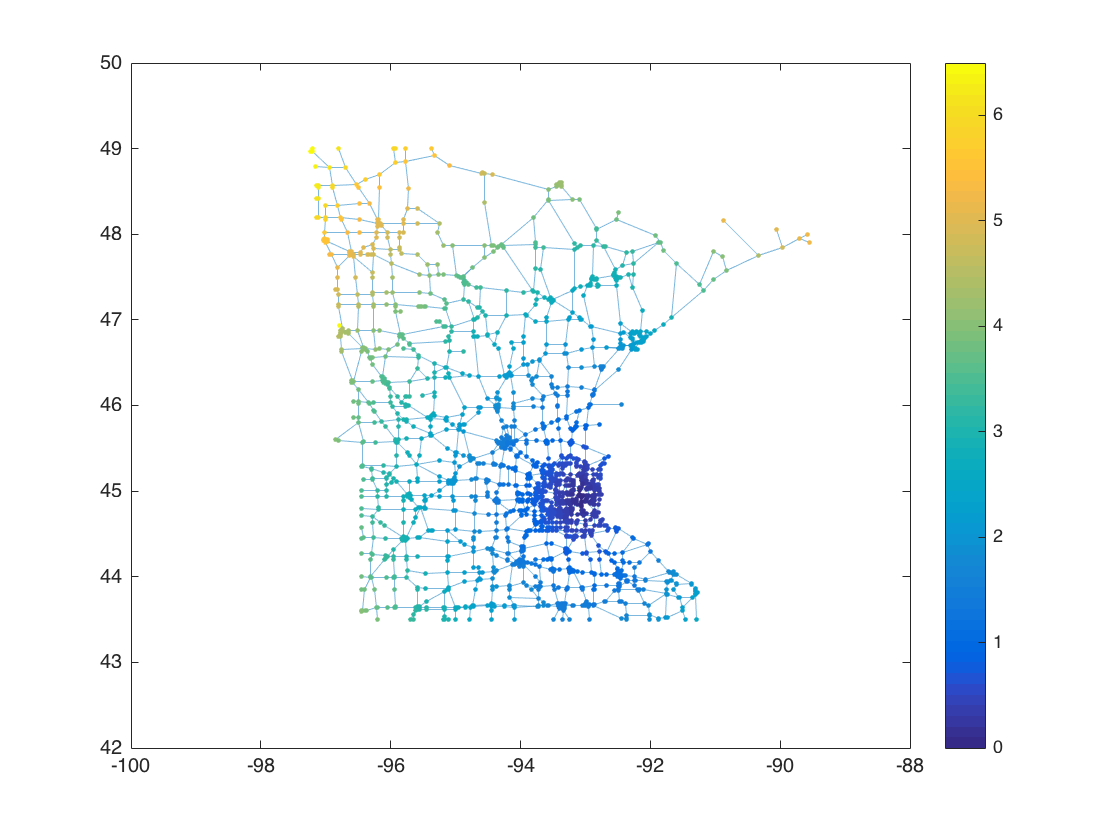
\includegraphics[width=1\textwidth]{abb1.png}
		\caption{amazing network}
		\label{img:abb1}
		\end{figure}\par\blindtext

	\subsection{Third subsection}	
		\blindtext

%% Zweiter Abschnitt
\section{Second section}
	\blindtext
	\subsection{First subsection}
		\Blindtext
		\begin{figure}[h]
		\centering
		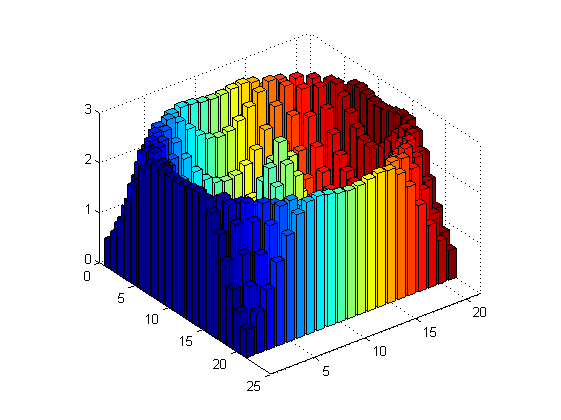
\includegraphics[width=1\textwidth]{abb2.png}
		\caption{flow distro}
		\label{img:abb2}
		\end{figure}\par\blindtext

%% Fazit
\section{Fazit}
	\blindtext
	

%% Deckblatt Anhang
\begin{titlepage}
	\section*{}
	%\addtocontents{toc}{\huge\bfseries \InsertTitle \par}
	%\renewcommand{\cftsecfont}{\scshape}
	\addtocontents{toc}{\cftpagenumbersoff{section}}
	\renewcommand\cftsecfont{\scshape}
	\addcontentsline{toc}{section}{Anhang}	
	\addtocontents{toc}{\cftpagenumberson{section}}
	\pagenumbering{Roman}
	\centering
	\vspace{3cm}
	{\huge\bfseries Anhang \par}
	
	\vfill
\end{titlepage}

%% Anhang
\appendix


%% Hintergrund
\section{Hintergrund}
	\blindtext
	\subsection{Hintergrund A}
		\blindtext


 \begin{table}[h!]
\setlength{\arrayrulewidth}{0.5mm}
\setlength{\tabcolsep}{18pt}
\renewcommand{\arraystretch}{1.5}
 
\newcolumntype{s}{>{\columncolor[HTML]{AAACED}} p{3cm}}
 
\arrayrulecolor[HTML]{000000}
 
\begin{tabular}{ |s|p{3cm}|p{3cm}|  }
\hline
\rowcolor{lightgray} \multicolumn{3}{|c|}{Country List} \\
\hline
Country Name    or Area Name& ISO ALPHA 2 Code &ISO ALPHA 3 \\
\hline
Afghanistan & AF &AFG \\
\rowcolor{gray}
Aland Islands & AX & ALA \\
Albania   &AL & ALB \\
Algeria  &DZ & DZA \\
American Samoa & AS & ASM \\
Andorra & AD & \cellcolor[HTML]{AA0044} AND    \\
Angola & AO & AGO \\
\hline
\end{tabular}
	
\caption{This table shows more  data}
\label{tab:mysecondtable}



\end{table}
\par
\blindtext
	\subsection{Hintergrund  B}
		here comes a citation \cite{greenwade93}
		\Blindtext

%% Quellverzeichnis
\newpage
\section{Quellenverzeichnis}
	\let\oldaddcontentsline\addcontentsline% Store \addcontentsline
	\renewcommand{\addcontentsline}[3]{}% Make \addcontentsline a no-op
	\begingroup
	\renewcommand{\section}[2]{}%%\renewcommand{\chapter}[2]{}% for other classes
		\bibliographystyle{plain}		
		\bibliography{my}
	\endgroup
	\let\addcontentsline\oldaddcontentsline% Restore \addcontentsline
%% Abbildungsverzeichnis
\section*{}
	\addcontentsline{toc}{section}{Abbildungsverzeichnis}	
	\listoffigures
\section*{}
	\addcontentsline{toc}{section}{Tabellenverzeichnis}
	\listoftables



\end{document}